\documentclass[11pt,a4paper]{article}

% Packages
\usepackage[utf8]{inputenc}
\PassOptionsToPackage{hyphens}{url}
\usepackage{amsmath,amssymb,amsthm}
\usepackage{mathtools}
\usepackage{graphicx}
\usepackage{booktabs}
\usepackage{array}
\usepackage[hypertexnames=false,hidelinks,pdfauthor={Kyle Elliott Mathewson},pdftitle={Moments of Magic Squares: Line-Sum Conditions, a Permutation Threshold, and Random Energies}]{hyperref}
\usepackage{geometry}
\usepackage{float}

% Reference helpers: the label prefix (fig:, thm:, sec:, ...) determines the name.
\makeatletter
\def\Cref@getprefix#1:#2\relax{#1}
\def\Cref@prefix@sec{sec}
\def\Cref@prefix@fig{fig}
\def\Cref@prefix@tab{tab}
\def\Cref@prefix@eq{eq}
\def\Cref@prefix@thm{thm}
\def\Cref@prefix@prop{prop}
\def\Cref@prefix@lem{lem}
\def\Cref@prefix@cor{cor}
\def\Cref@prefix@conj{conj}
\def\Cref@prefix@def{def}
\def\Cref@prefix@rem{rem}
\def\Cref@prefix@ex{ex}

\def\Cref@type@cap#1{%
  \edef\Cref@tmp{#1}%
  \ifx\Cref@tmp\Cref@prefix@sec Section%
  \else\ifx\Cref@tmp\Cref@prefix@fig Figure%
  \else\ifx\Cref@tmp\Cref@prefix@tab Table%
  \else\ifx\Cref@tmp\Cref@prefix@eq Equation%
  \else\ifx\Cref@tmp\Cref@prefix@thm Theorem%
  \else\ifx\Cref@tmp\Cref@prefix@prop Proposition%
  \else\ifx\Cref@tmp\Cref@prefix@lem Lemma%
  \else\ifx\Cref@tmp\Cref@prefix@cor Corollary%
  \else\ifx\Cref@tmp\Cref@prefix@conj Conjecture%
  \else\ifx\Cref@tmp\Cref@prefix@def Definition%
  \else\ifx\Cref@tmp\Cref@prefix@rem Remark%
  \else\ifx\Cref@tmp\Cref@prefix@ex Example%
  \else Ref.%
  \fi\fi\fi\fi\fi\fi\fi\fi\fi\fi\fi\fi
}

\def\Cref@type@low#1{%
  \edef\Cref@tmp{#1}%
  \ifx\Cref@tmp\Cref@prefix@sec section%
  \else\ifx\Cref@tmp\Cref@prefix@fig figure%
  \else\ifx\Cref@tmp\Cref@prefix@tab table%
  \else\ifx\Cref@tmp\Cref@prefix@eq equation%
  \else\ifx\Cref@tmp\Cref@prefix@thm theorem%
  \else\ifx\Cref@tmp\Cref@prefix@prop proposition%
  \else\ifx\Cref@tmp\Cref@prefix@lem lemma%
  \else\ifx\Cref@tmp\Cref@prefix@cor corollary%
  \else\ifx\Cref@tmp\Cref@prefix@conj conjecture%
  \else\ifx\Cref@tmp\Cref@prefix@def definition%
  \else\ifx\Cref@tmp\Cref@prefix@rem remark%
  \else\ifx\Cref@tmp\Cref@prefix@ex example%
  \else ref.%
  \fi\fi\fi\fi\fi\fi\fi\fi\fi\fi\fi\fi
}

\DeclareRobustCommand{\Cref}[1]{%
  \begingroup
  \edef\Cref@label{#1}%
  \edef\Cref@prefix{\expandafter\Cref@getprefix\Cref@label:\relax}%
  \hyperref[#1]{\Cref@type@cap{\Cref@prefix}~\ref*{#1}}%
  \endgroup
}
\DeclareRobustCommand{\cref}[1]{%
  \begingroup
  \edef\Cref@label{#1}%
  \edef\Cref@prefix{\expandafter\Cref@getprefix\Cref@label:\relax}%
  \hyperref[#1]{\Cref@type@low{\Cref@prefix}~\ref*{#1}}%
  \endgroup
}
\makeatother

\geometry{margin=0.9in}
\setlength{\emergencystretch}{2em} % reduce overfull lines without \sloppy
\setlength{\textfloatsep}{10pt plus 2pt minus 2pt}
\setlength{\intextsep}{8pt plus 2pt minus 2pt}
\setlength{\abovecaptionskip}{4pt}
% captions in \small
\makeatletter
\long\def\@makecaption#1#2{\vskip\abovecaptionskip\small\sbox\@tempboxa{#1: #2}\ifdim\wd\@tempboxa>\hsize #1: #2\par\else\global\@minipagefalse\hb@xt@\hsize{\hfil\box\@tempboxa\hfil}\fi\vskip\belowcaptionskip}
\makeatother
% Float placement parameters (reduce float-page waste)
\renewcommand{\topfraction}{0.9}
\renewcommand{\bottomfraction}{0.6}
\renewcommand{\textfraction}{0.07}
\renewcommand{\floatpagefraction}{0.85}
\setcounter{topnumber}{3}
\setcounter{totalnumber}{5}

% Theorem environments
\theoremstyle{plain}
\newtheorem{theorem}{Theorem}[section]
\newtheorem{lemma}[theorem]{Lemma}
\newtheorem{proposition}[theorem]{Proposition}
\newtheorem{corollary}[theorem]{Corollary}
\newtheorem{conjecture}[theorem]{Conjecture}

\theoremstyle{definition}
\newtheorem{definition}[theorem]{Definition}
\newtheorem{example}[theorem]{Example}

\theoremstyle{remark}
\newtheorem{remark}[theorem]{Remark}

% Custom commands
\newcommand{\R}{\mathbb{R}}
\newcommand{\Z}{\mathbb{Z}}
\newcommand{\N}{\mathbb{N}}
\newcommand{\Cov}{\mathrm{Cov}}
\newcommand{\Var}{\mathrm{Var}}
\newcommand{\Efull}{E_{\mathrm{full}}}
\newcommand{\Efour}{E_4}
\newcommand{\E}{\mathbb{E}}
\newcommand{\tr}{\operatorname{tr}}


\title{\textbf{Moments of Magic Squares:\\ Line-Sum Conditions, a Permutation Threshold,\\ and Random Energies}}

\author{Kyle Elliott Mathewson\\
\textit{Faculty of Science, University of Alberta}\\
\texttt{kyle.mathewson@ualberta.ca}}

\date{\today}

\begin{document}

\maketitle

\begin{abstract}
Every semi-magic square of order $n$ satisfies the axial moment identities $\sum_{i,j}s_{ij}j^m=\sum_{i,j}s_{ij}i^m=M(n)\sum_jj^m$ for all $m\ge1$, where $M(n)=n(n^2+1)/2$. For real matrices the converse requires $1\le m\le n-1$, whereas for arrangements of $\{1,\dots,n^2\}$ fewer moments suffice once $n\ge14$. We define the \emph{permutation threshold} $k^*(n)$ as the least $k$ such that every arrangement satisfying these identities for $1\le m\le k$ is semi-magic. In terms of the column-sum deviations $\gamma_j$, the degree-$k$ conditions state that $\sum_j\gamma_jt^j$ is divisible by $(t-1)^{k+1}$, linking $k^*(n)$ to the Prouhet--Tarry--Escott problem. While Schur's bound on real zeros gives $k^*(n)\le\sqrt{2(n-1)\log(n^4/4)}$, we prove the converse realisability bound $k^*(n)\ge(\sqrt2-o(1))\sqrt n$ (and $k^*(n)\ge(\sqrt6-o(1))\sqrt n$ when $4\mid n$) by perturbing semi-magic squares with complementary row pairs via horizontal swaps. We also show that $k^*(n)=n-1$ for $3\le n\le13$, $k^*(n)=n-2$ for $14\le n\le17$, and $k^*(n)\le n-3$ for $n\ge18$, and determine $k^*(n)$ for $18\le n\le40$ with computer assistance. Finally, at the $k=1$ level of the hierarchy, we specialise the Mantel--Hubert quadratic assignment variance formula to obtain exact means, variances, and limit laws under a uniform random arrangement for the full line-sum energy $\Efull$, for the four-term energy $\Efour$ combining the first moments and the two diagonals, and for Loly's moment of inertia, and find that $|L_4|=14{,}639{,}440$ arrangements of order $4$ satisfy $\Efour=0$.

\medskip
\noindent\textbf{Keywords:} magic squares, Prouhet--Tarry--Escott problem, polynomials with integer coefficients, permutation statistics, combinatorial central limit theorem, moment of inertia

\noindent\textbf{MSC 2020:} 05B20 (primary); 05A05, 11C08, 60C05, 60F05
\end{abstract}


\section{Introduction}
\label{sec:introduction}

Magic squares are among the oldest objects of recreational mathematics: the $3\times3$ Lo Shu appears in Chinese sources more than two millennia old, a $4\times4$ square is engraved in D\"urer's \emph{Melencolia~I} (1514), and systematic constructions for every order have been known since the seventeenth century \cite{andrews1960magic,pickover2002zen}.
The modern literature treats them from several directions: enumeration and the geometry of the associated polytopes \cite{stanley1973magic,ehrhart1973magic,ahmed2003polyhedral,beck2006insideout,beck2010enumeration}, spectral and matrix properties \cite{loly2009spectra,nordgren2012properties,nordgren2014spectra,cameron2013signatura}, and, in work of Loly and collaborators, physical invariants such as the moment of inertia and the multipole moments \cite{loly2004invariance,rogers2004inertia,rogers2005multipole}.

\begin{definition}[Magic square]
\label{def:magic_square}
An \emph{arrangement} of order $n$ is a bijection $S=(s_{ij})$ from the cells of the $n\times n$ grid onto $\{1,\dots,n^2\}$.
It is a \emph{magic square} if every row, every column and both main diagonals sum to the magic constant $M(n)=n(n^2+1)/2$, and \emph{semi-magic} if only the rows and columns do.
\end{definition}

This paper reads an arrangement as a function on the grid: the centred entry $z_{ij}=s_{ij}-(n^2+1)/2$ is a \emph{height} over the centred cell $(x_{ij},y_{ij})=(j-\frac{n-1}2,\ \frac{n-1}2-i)$ (\Cref{def:coords}).
The points $(x_{ij},y_{ij},z_{ij})\in\R^3$ have a convex hull, studied in the companion paper~A \cite{mathewson_gems}; here the object is the height function $z$ alone.
Every line-sum condition ``row $k$ sums to $M(n)$'' becomes ``$z$ is orthogonal to the centred indicator of row $k$'', i.e.\ $\Cov(R_k,Z)=0$ for the empirical covariance over the $n^2$ cells.
A magic square is therefore an arrangement whose height function is orthogonal to a fixed $2n$-dimensional space $W$ of test functions, and the \emph{energy} $\Efull(S)=\sum_L\Cov(\mathbf 1_L,Z)^2$ over the $2n+2$ lines vanishes exactly on magic squares (\Cref{lem:zero_set}).
This is a reformulation of the definition, not a theorem about magic squares (\Cref{rem:tautology}); its value is that it makes certain questions natural, and the paper is organised around their answers.

\paragraph{Contributions.}
\begin{enumerate}\setlength\itemsep{1pt}
\item \emph{The moment hierarchy} (\Cref{prop:hierarchy}, \Cref{thm:perm_threshold}). Replacing the line indicators by the polynomial test functions $x^m,y^m$ gives, for each degree $k$, the conditions $\Cov(X^m,Z)=\Cov(Y^m,Z)=0$ for $m\le k$. For real-valued height functions these are equivalent to equal row and column sums if and only if $k\ge n-1$ (a Vandermonde fact). For permutations of $1,\dots,n^2$, integrality and the bound on line sums lower the threshold $k^*(n)$ to at most $n-2$ for every $n\ge14$, whereas $k^*(n)=n-1$ for $3\le n\le13$ (computer-verified witnesses, \Cref{rem:kstar_search}). The four-term energy $\Elow$ is the degree-one truncation. Loly's invariance of the moment of inertia \cite{loly2004invariance} is the single condition $\Cov(Z,X^2+Y^2)=0$, implied by the degree-two conditions but much weaker than them (\Cref{cor:loly}); the same identity gives the null distribution of the moment of inertia of a random arrangement (\Cref{cor:loly_null}).
\item \emph{Balance of the signed mass} (\Cref{sec:balance}). $\Efull=0$ is equivalent to $\sum_cz_c\varphi_c=0$ for every $\varphi$ in the line space (\Cref{thm:linear_balance}); this contains Loly's invariant, the vanishing of the centre of mass and of all axial moments, and leaves the mixed moments free. For any arrangement, $|\sum_cz_c(x_c,y_c)|^2\le N^2\frac{n(n^2-1)}{12}\Efull$ with a sharp constant (\Cref{thm:quant_balance}). The corresponding statement for unit vectors is false: the eight $3\times3$ magic squares all have a ring imbalance $2(2-\sqrt2)\sqrt5$, and a three-dimensional unit-vector sum never vanishes (\Cref{prop:unit_negative}); a numerical comparison for $n=4$ is given in \Cref{tab:unit_n4}.
\item \emph{Exact statistics of a random arrangement} (\Cref{prop:random_energy_moments}). $\E[\Elow]=(n^2+1)(n^4-n^2+12n-12)/(72n^2)$ and $\E[\Efull]=(n^4-1)/(6n^2)$, with exact variances; $\Elow/\E[\Elow]\to\mathrm{Exp}(1)$ by Hoeffding's combinatorial central limit theorem. Monte Carlo with $10^8$ samples per order agrees for $3\le n\le 8$ to within $5\times10^{-4}$ relative error.
\item \emph{The single-swap formula} (\Cref{thm:swap}). Exchanging two entries of a magic square that differ by $d$ raises $\Efull$ by exactly $d^2m/n^4$, where $m\in\{2,\dots,6\}$ counts the lines separating the two cells; every magic square is a strict local minimum, with minimum gap between $2/n^4$ and $6/n^4$. Elementary steepest descent and annealing on $\Efull$ are reported in \Cref{sec:algorithms}.
\item \emph{The low-mode class for $n=4$} (\Cref{prop:L4}). Exactly $14{,}639{,}440$ of the $16!$ arrangements satisfy $\Elow=0$, of which $7{,}040$ are magic; the count is a meet-in-the-middle enumeration and agrees with a Gaussian local-limit estimate to within $20\%$.
\end{enumerate}

\paragraph{Context and scope.}
The enumerative and polyhedral theory of magic squares is classical. Nonnegative integer matrices with all line sums equal to $t$ are the lattice points of the $t$-th dilate of the Birkhoff polytope and their number is a polynomial in $t$ \cite{stanley1973magic,ehrhart1973magic}; the count of magic squares with distinct entries is an Ehrhart quasi-polynomial of an inside-out polytope \cite{beck2006insideout,beck2010enumeration}; the cones of magic squares and cubes have Hilbert-basis descriptions \cite{ahmed2003polyhedral}; and arrays with fixed margins have been studied as a sample space by Diaconis and Gangolli \cite{diaconis1995rectangular}.
None of this is used or extended here: our sample space is the uniform distribution on permutations, and we count nothing polyhedrally.
The orthogonality reading is elementary and implicit in Loly's work: he derived the invariance of the moment of inertia from row and column sums alone \cite{loly2004invariance}, and Rogers and Loly studied the multipole expansion of a magic cube \cite{rogers2005multipole}.
The linear balance statements of \Cref{sec:balance} belong to that circle of ideas; what we add is their formulation as a single orthogonality statement, the sharp quantitative bound, and the negative results for nonlinear (unit-vector) balance.
The Vandermonde threshold of the hierarchy is elementary linear algebra.
To our knowledge the permutation refinement (\Cref{thm:perm_threshold}), the exact moments and limit law for random arrangements, the swap formula and the exact count for $n=4$ are new; they are small statements about a classical object, and we make no claim that the energy reformulation by itself is a result.

\paragraph{Organisation.}
\Cref{sec:background} fixes coordinates and collects the facts used; \Cref{sec:theory} contains the projection lemma, the hierarchy and the swap formula; \Cref{sec:balance} the balance results; \Cref{sec:results} the computations; \Cref{sec:discussion} what the viewpoint does and does not buy, local search, and open questions; the appendices the methods, the variance closed forms and a witness for $k^*(5)=4$.


\section{Background}
\label{sec:background}

\subsection{Centred coordinates and the height function}
\label{sec:bg_coords}

Let $S=(s_{ij})$ be an arrangement of order $n$, with cells indexed by $i,j\in\{0,\dots,n-1\}$ ($i$ the row from the top, $j$ the column from the left), and write $N=n^2$.

\begin{definition}[Centred coordinates and height function]
\label{def:coords}
To the cell $(i,j)$ assign
\begin{equation}
x_{ij}=j-\frac{n-1}{2},\qquad y_{ij}=\frac{n-1}{2}-i,\qquad z_{ij}=s_{ij}-\frac{N+1}{2}.
\label{eq:coords}
\end{equation}
The function $z=(z_{ij})$ on the grid is the \emph{height function} of $S$.
\end{definition}

The horizontal coordinates centre the grid at the origin; the vertical coordinate centres the entries so that the mean entry $(N+1)/2$ sits at height zero.
All three have mean zero over the $N$ cells (\Cref{lem:variances}).
The $N$ points $(x_{ij},y_{ij},z_{ij})\in\R^3$ have a convex hull, the object of the companion paper~A, \emph{Magic Gems: A Polyhedral Framework for Magic Squares} (Mathewson, arXiv:2512.09170) \cite{mathewson_gems}, which studies the convex hull of these points, the symmetry classification of the $880$ order-four hulls, and the hulls of Siamese squares.
Nothing below uses the hull.

\subsection{Covariance and Loly's planar moment}
\label{sec:bg_cov}

For functions $\varphi,f$ on the cells, $\Cov(\varphi,f)$ denotes the empirical covariance over the $N$ cells, $\Cov(\varphi,f)=\frac1N\sum_c(\varphi_c-\bar\varphi)(f_c-\bar f)$, and $X,Y,Z$ denote the functions \eqref{eq:coords}.
Loly's planar moment of inertia \cite{loly2004invariance} places the \emph{value} $s_{ij}$ as a mass at the planar point $(x_{ij},y_{ij})$ and computes $\sum s_{ij}(x_{ij}^{2}+y_{ij}^{2})$.
It is an affine function of the single degree-two cross-moment $\Cov(Z,X^2+Y^2)$ (\Cref{cor:loly}).

\subsection{Two tools from permutation statistics}
\label{sec:bg_perm}

Let $\pi$ be a uniformly random permutation of $\{1,\dots,N\}$ and $a,b\in\R^N$ fixed vectors.
The quantity $T_a=\sum_i a_i b_{\pi(i)}$ is a \emph{linear permutation statistic}.
Its mean is $N\bar a\bar b$ and, for two such statistics with the same $b$ (Wald--Wolfowitz \cite{waldwolfowitz1944}, polarised),
\begin{equation}
\Cov(T_a,T_{a'})=\frac{1}{N-1}\sum_i(a_i-\bar a)(a'_i-\bar a')\sum_j(b_j-\bar b)^2 .
\label{eq:ww_identity}
\end{equation}
Hoeffding's combinatorial central limit theorem \cite[Thm.~3]{hoeffding1951} gives asymptotic normality of $\sum_i c_N(i,\pi(i))$ when, for every integer $r\ge3$, $N^{-1}\sum_{i,j}|d_N(i,j)|^r$ is $O\bigl((N^{-1}\sum_{i,j}d_N(i,j)^2)^{r/2}\bigr)$, $d_N$ being the doubly centred array; for product arrays $c_N(i,j)=a_ib_j$ the condition reduces to a bound on the standardised absolute moments of $a$ and $b$.
In \Cref{sec:random_energy} the energies of a random arrangement are quadratic forms in such statistics; \eqref{eq:ww_identity} gives their means exactly, and the distribution of a quadratic form in Gaussian variables can be computed by numerical inversion of its characteristic function, as in Imhof's method \cite{imhof1961}.

\subsection{Enumeration and related polytopes}
\label{sec:bg_polytopes}

There are $8$ magic squares of order $3$, all images of the Lo Shu under the dihedral group $D_4$ of the square; $7{,}040$ of order $4$, forming $880$ $D_4$-orbits first listed by Fr\'enicle de Bessy and verified many times since \cite{beck2010enumeration}; and $275{,}305{,}224$ of order $5$ \cite{gardner1976}.
For $n\ge6$ only statistical estimates are known \cite{trump2012enumeration}.
Classical constructions show that magic squares exist for all $n\ge3$ \cite{andrews1960magic}.

The polytope literature concerns a different object from the one used here.
An $n\times n$ nonnegative integer matrix with all row and column sums equal to $t$ is a lattice point of the $t$-th dilate of the Birkhoff polytope, and their number is a polynomial in $t$ \cite{stanley1973magic,ehrhart1973magic,ziegler1995lectures}; adding the diagonal conditions and distinct entries leads to the inside-out polytopes of Beck and Zaslavsky \cite{beck2006insideout,beck2010enumeration}; the cones of magic squares and cubes have Hilbert-basis descriptions \cite{ahmed2003polyhedral}; and contingency tables with fixed margins are the same lattice points studied as a sample space \cite{diaconis1995rectangular}.
Spectral and matrix properties of a magic square \cite{loly2009spectra,nordgren2012properties,nordgren2014spectra}, the singular-value signatures of Cameron, Rogers and Loly \cite{cameron2013signatura}, and Loly's physical invariants \cite{loly2004invariance,rogers2004inertia,rogers2005multipole,loly2007franklin} are closer to our viewpoint: they attach a quantity to one square and ask what it reveals.


\section{The moment hierarchy and the permutation threshold}
\label{sec:theory}

\subsection{Moment conditions}
\label{sec:theory_hierarchy}

For a centred $f\in\mathcal F$ let $\gamma_j(f)=\sum_if_{ij}$ and $\rho_i(f)=\sum_jf_{ij}$ be its column and row sums; for $f=z(S)$ these are the deviations $\gamma,\rho$ of $S$.
For $\gamma\in\R^n$ put $P_\gamma(t)=\sum_{j=0}^{n-1}\gamma_jt^j$.

\begin{definition}[Degree-$k$ conditions]
\label{def:degree_k}
A centred $f\in\mathcal F$ satisfies the \emph{degree-$k$ conditions} ($k\ge1$) if $\langle x^{m},f\rangle=\langle y^{m},f\rangle=0$ for $1\le m\le k$.
For $f=z(S)$ these read $\sum_{i,j}z_{ij}x_j^m=\sum_{i,j}z_{ij}y_i^m=0$, i.e.\ $\Cov(X^m,Z)=\Cov(Y^m,Z)=0$.
\end{definition}

\begin{lemma}[Polynomial form]
\label{lem:poly_form}
If $\varphi$ depends only on the column index, $\langle\varphi,f\rangle=\frac1N\sum_j\varphi(j)\gamma_j(f)$; similarly for rows.
For $\gamma\in\R^{n}$ and $k\ge0$ the following are equivalent:
(i)~$\sum_jx_j^{m}\gamma_j=0$ for $0\le m\le k$;
(ii)~$\sum_j\binom{j}{r}\gamma_j=0$ for $0\le r\le k$;
(iii)~$(t-1)^{k+1}$ divides $P_\gamma(t)$.
Hence a centred $f$ satisfies the degree-$k$ conditions if and only if $(t-1)^{k+1}$ divides both $P_{\gamma(f)}$ and $P_{\rho(f)}$.
\end{lemma}

\begin{proof}
The first statement is $\sum_{i,j}\varphi(j)f_{ij}=\sum_j\varphi(j)\gamma_j(f)$.
The families $(x_j^{m})_{m\le k}$ and $(\binom{j}{r})_{r\le k}$ both span the restrictions to $\{0,\dots,n-1\}$ of the polynomials of degree at most $k$ in $j$, so (i)$\Leftrightarrow$(ii); and $P_\gamma(t)=\sum_{r}\bigl(\sum_j\binom jr\gamma_j\bigr)(t-1)^{r}$ is the Taylor expansion at $t=1$, so (ii)$\Leftrightarrow$(iii).
The case $m=0$ of (i) holds for every centred $f$.
\end{proof}

\begin{proposition}[Moment hierarchy]
\label{prop:hierarchy}
Let $n\ge3$ and let $f\in\mathcal F$ be centred.
\begin{enumerate}
\item[(a)] If $\gamma(f)=\rho(f)=0$, then $\langle a(X)+b(Y),f\rangle=0$ for all functions $a,b$ on $\{x_0,\dots,x_{n-1}\}$; in particular $f$ satisfies the degree-$k$ conditions for every $k$.
For $f=z(S)$ with $S$ magic, also $\langle a(X)+b(Y)+c_1\mathbf 1_{D_{\mathrm m}}+c_2\mathbf 1_{D_{\mathrm a}},z\rangle=0$.
\item[(b)] If $k\ge n-1$, the degree-$k$ conditions imply $\gamma(f)=\rho(f)=0$.
\item[(c)] If $1\le k\le n-2$, the function $f_{ij}=\frac1n(-1)^{j}\binom{k+1}{j}$ ($0\le j\le k+1$), $f_{ij}=0$ ($j>k+1$), satisfies the degree-$k$ conditions but not the degree-$(k+1)$ conditions, and $\gamma(f)\ne0$.
\end{enumerate}
\end{proposition}

\begin{proof}
(a) is the first statement of \Cref{lem:poly_form}.  (b) A nonzero polynomial of degree at most $n-1$ is not divisible by $(t-1)^{n}$.  (c) Here $\rho(f)=0$ and $P_{\gamma(f)}(t)=(1-t)^{k+1}$.
\end{proof}

Part (a) contains the vanishing of the centre of mass $\sum_cz_c(x_c,y_c)$ and of all axial moments $\sum_cz_cx_c^m$, $\sum_cz_cy_c^m$ of a semi-magic square, in the spirit of the multipole analysis of a magic cube by Rogers and Loly \cite{rogers2005multipole}.
Parts (b) and (c) are the invertibility of a Vandermonde matrix.
The mixed moments are not determined by the line sums:

\begin{remark}[Mixed moments]
\label{rem:product_inertia}
The magic square with rows $(1,6,11,16)$, $(8,15,2,9)$, $(12,3,14,5)$, $(13,10,7,4)$ has $\sum_cz_cx_cy_c=60$.
Among the $880$ magic squares of order $4$ up to $D_4$, the product of inertia $\sum_cz_cx_cy_c$ is nonzero for $824$, takes $48$ distinct absolute values between $0$ and $60$, and $\sum_cz_cx_c^2y_c$, $\sum_cz_cx_cy_c^2$ are nonzero for $623$ and $773$ of them.
For $n=3$ the mixed moment $\sum_cz_cx_cy_c$ vanishes for all eight magic squares, because $s_c+s_{-c}=10$ for centrally opposite cells, so $z$ is odd under $(x,y)\mapsto(-x,-y)$ while $xy$ is even.
\end{remark}

\begin{corollary}[Loly's invariant {\cite{loly2004invariance}}]
\label{cor:loly}
Let $I(S)=\sum_{i,j}s_{ij}(x_{j}^{2}+y_{i}^{2})$ be the moment of inertia about the centre of the masses $s_{ij}$ placed at $(x_j,y_i)$.  For every arrangement,
\begin{equation}
I(S)=N\,\Cov\bigl(Z,\,X^{2}+Y^{2}\bigr)+\frac{n^{2}(n^{4}-1)}{12}
=\sum_j x_j^{2}\gamma_j+\sum_i y_i^{2}\rho_i+\frac{n^{2}(n^{4}-1)}{12}.
\label{eq:loly_identity}
\end{equation}
Hence $I(S)=n^{2}(n^{4}-1)/12$ if and only if the single condition $\Cov(Z,X^{2}+Y^{2})=0$ holds; it is implied by the degree-$2$ conditions, hence by the semi-magic property.
\end{corollary}

\begin{proof}
Substitute $s_{ij}=z_{ij}+\frac{N+1}2$ and use \Cref{lem:variances} and \Cref{lem:poly_form}: $\frac{N+1}2\sum_{i,j}(x_j^{2}+y_i^{2})=\frac{N+1}2\cdot\frac{n^{2}(n^{2}-1)}{6}$.
\end{proof}

Loly's derivation uses the row and column sums in the same way \cite{loly2004invariance}.
The single condition is much weaker than the degree-$2$ conditions: for $n=3$, $24{,}192$ of the $9!$ arrangements have $I=60$, while $72$ (the semi-magic squares, \Cref{rem:n3_lowmode}) satisfy the degree-$2$ conditions.
The energy $\Elow$ of \eqref{eq:Elow} combines the degree-$1$ conditions with the two diagonal conditions: $\Elow=\langle x,z\rangle^2+\langle y,z\rangle^2+(\delta_{\mathrm m}^2+\delta_{\mathrm a}^2)/N^2$.

\subsection{The permutation threshold}
\label{sec:kstar}

By \Cref{prop:hierarchy}, for real-valued $f$ the degree-$k$ conditions force equal row and column sums exactly when $k\ge n-1$.
For arrangements the deviations are integers of bounded size, and the threshold drops.

\begin{definition}
\label{def:kstar}
For $n\ge3$, $k^*(n)$ is the least $k\ge1$ such that every arrangement of order $n$ satisfying the degree-$k$ conditions is semi-magic.
\end{definition}

By \Cref{prop:hierarchy}(b), $k^*(n)\le n-1$.
By \Cref{lem:poly_form}, an arrangement satisfies the degree-$k$ conditions if and only if $\gamma$ and $\rho$ lie in the lattice
\[
\Lambda_{n,k}=\{\gamma\in\Z^{n}:(t-1)^{k+1}\mid P_\gamma(t)\}=(t-1)^{k+1}\,\Z[t]_{<n-k-1},
\]
of rank $n-k-1$.
Writing $\gamma=\gamma^+-\gamma^-$ with $\gamma^\pm\ge0$, the condition $\gamma\in\Lambda_{n,k}$ says that the multisets in which $j$ occurs $\gamma^+_j$, resp.\ $\gamma^-_j$, times have equal power sums of degrees $0,\dots,k$: a Prouhet--Tarry--Escott system \cite{wright1959prouhet,borwein2002computational}.
Small vectors in $\Lambda_{n,k}$ are classical: the Prouhet--Thue--Morse vector $\bigl((-1)^{s_2(j)}\bigr)_{0\le j<2^{k+1}}$ ($s_2$ the binary digit sum) has entries $\pm1$ and lies in $\Lambda_{2^{k+1},k}$ \cite{wright1959prouhet,allouche1999ubiquitous}, and Borwein, Erd\'elyi and K\'os construct polynomials of degree $n$ with coefficients in $\{-1,0,1\}$ vanishing to order $\ge c\sqrt{n/\log n}$ at $1$ \cite[Thm.~2.7]{BEK1999}.
The question is therefore how large $k$ can be for vectors that are column-deviation vectors of arrangements.

\begin{theorem}[The permutation threshold]
\label{thm:perm_threshold}
\leavevmode
\begin{enumerate}
\item[(a)] For all $n\ge3$, $\displaystyle k^{*}(n)\le\Bigl\lfloor\sqrt{\pi e\,(n-1)\log(n^{4}/4)}\Bigr\rfloor\le 2\sqrt{\pi e}\,\sqrt{n\log n}$.
\item[(b)] $\displaystyle\liminf_{n\to\infty}\frac{k^{*}(n)}{\sqrt n}\ge\sqrt2$.
\item[(c)] $k^{*}(n)=n-1$ for $3\le n\le13$, $k^{*}(n)=n-2$ for $14\le n\le17$, and $k^{*}(n)\le n-3$ for every $n\ge18$.  The values for $14\le n\le40$ are those of \Cref{tab:kstar}.
\end{enumerate}
\end{theorem}

The constant $2\sqrt{\pi e}$ is about $5.84$.
Part (a) improves on $k^*(n)\le n-3$ only for $n\ge166$; for smaller $n$ the exact computation behind (c) is much stronger (\Cref{fig:kstar}).
Parts (c) for $n\ge14$ and the values in \Cref{tab:kstar} rest on exact computer calculations, described in \Cref{sec:kstar_exact}.

\subsection{Proof of the upper bound}
\label{sec:kstar_upper}

\begin{lemma}[Column feasibility]
\label{lem:col_feasible}
Let $\gamma$ be the column-deviation vector of an arrangement.  For every set $J$ of $p$ columns,
\begin{equation}
\Bigl|\sum_{j\in J}\gamma_j\Bigr|\le \frac{pn(N-pn)}{2}.
\label{eq:col_feasible}
\end{equation}
In particular $|\gamma_j|\le n^{2}(n-1)/2$, $\|\gamma\|_1\le N^{2}/4$ and $\|\gamma\|_2^2\le n^5(n^2-1)/12$.  The same holds for $\rho$.
\end{lemma}

\begin{proof}
The $pn$ cells of $J$ carry distinct values, whose sum is at most that of the $pn$ largest values, $pn(2N-pn+1)/2$; subtracting $pM(n)=pn(N+1)/2$ gives the upper bound, and the lower bound is symmetric.
With $p$ the number of positive $\gamma_j$, $\|\gamma\|_1=2\sum_{\gamma_j>0}\gamma_j\le pn(N-pn)\le N^2/4$.
Finally \eqref{eq:col_feasible} says that $\gamma$ is majorised by the vector with entries $n(N-(2p-1)n)/2$, $1\le p\le n$, whose squared norm is $n^5(n^2-1)/12$, and $\|\cdot\|_2^2$ is Schur-convex.
\end{proof}

\begin{lemma}[Order of vanishing of an integer polynomial at $1$]
\label{lem:jensen}
Let $\gamma\in\Z^{n}\setminus\{0\}$ with $(t-1)^{K}\mid P_\gamma$ for some $K\ge1$.  Then $K^{2}\le \pi e\,(n-1)\log\|\gamma\|_1$.
\end{lemma}

\begin{proof}
Write $P=P_\gamma$ and $L=\|\gamma\|_1$; note $K\le\deg P\le n-1$.
Since $P$ has integer coefficients and leading coefficient $a\ne0$, Jensen's formula gives
$\int_{-1/2}^{1/2}\log|P(e^{2\pi i\theta})|\,d\theta=\log\bigl(|a|\prod_\alpha\max(1,|\alpha|)\bigr)\ge0$, the product over the roots of $P$.
On $|z|=1$ we have $|P(z)|\le L$.
Since $P^{(i)}(1)=0$ for $i<K$, Taylor's formula with integral remainder along the segment $[1,z]$, which lies in the closed unit disc when $|z|=1$, gives
\[
|P(z)|\le\frac{|z-1|^{K}}{K!}\max_{|w|\le1}|P^{(K)}(w)|\le L\binom{n-1}{K}|z-1|^{K}\le L\Bigl(\frac{e(n-1)|z-1|}{K}\Bigr)^{K},
\]
because $|P^{(K)}(w)|\le\sum_j|\gamma_j|\,j(j-1)\cdots(j-K+1)$ for $|w|\le1$.
With $|e^{2\pi i\theta}-1|\le2\pi|\theta|$ and $\beta=2\pi e(n-1)/K\ge2\pi e$ we get $\log|P(e^{2\pi i\theta})|\le\log L+K\log\min(1,\beta|\theta|)$, and
$\int_{-1/2}^{1/2}\log\min(1,\beta|\theta|)\,d\theta=-2/\beta$.
Hence $0\le\log L-2K/\beta=\log L-K^{2}/(\pi e(n-1))$.
\end{proof}

\begin{proof}[Proof of \Cref{thm:perm_threshold}(a)]
Let $S$ satisfy the degree-$k$ conditions with $(k+1)^2>\pi e(n-1)\log(n^4/4)$.
If $\gamma\ne0$, then $(t-1)^{k+1}\mid P_\gamma$ (\Cref{lem:poly_form}) and $\|\gamma\|_1\le n^4/4$ (\Cref{lem:col_feasible}), contradicting \Cref{lem:jensen}.
So $\gamma=0$, and likewise $\rho=0$.
The second inequality follows from $(n-1)\log(n^4/4)<4n\log n$.
\end{proof}

The order $\sqrt{n\log n}$ also follows from \cite[Thm.~2.1]{BEK1999}, applied to $P_\gamma(t)/(t^{r}\max_j|\gamma_j|)$ with $r$ the index of the first nonzero $\gamma_j$; that theorem bounds the number of zeros at $1$ of $\sum_{j\le n}a_jt^j$ with $|a_j|\le1$ by $c\sqrt{n(1-\log|a_0|)}$, with an unspecified absolute constant.
\Cref{lem:jensen} is a self-contained version for integer coefficients.
An argument using only that $\gamma$ is a nonzero integer vector with $\|\gamma\|_\infty\le n^3$ cannot give an upper bound of smaller order than $\sqrt n$: the box principle applied to the vectors in $\{0,\dots,n^3\}^n$ and their binomial moments of order $<K$ produces such vectors in $\Lambda_{n,K-1}$ with $K\asymp\sqrt n$.

\subsection{Proof of the lower bound}
\label{sec:kstar_lower}

A lower bound $k^*(n)\ge K$ requires an arrangement that satisfies the degree-$(K-1)$ conditions without being semi-magic.
We keep all row sums equal to $M(n)$ and control the column deviations by swaps.

\begin{definition}
Rows $i\ne i'$ of an arrangement are \emph{twins on} a set $J$ of columns if $s_{ij}+s_{i'j}=N+1$ for all $j\in J$.
\end{definition}

\begin{lemma}[Twin swaps]
\label{lem:twin}
Let $S$ be semi-magic, let rows $i,i'$ be twins on $J$, let $j,j'\in J$ and $d=s_{ij'}-s_{ij}$.
Exchanging the entries of row $i$ in columns $j,j'$ changes the column deviations by $d(e_j-e_{j'})$, exchanging those of row $i'$ changes them by $-d(e_j-e_{j'})$, and neither changes a row sum.
Exchanges involving pairwise disjoint sets of cells can be combined, and their effects add.
\end{lemma}

\begin{proof}
$s_{i'j}-s_{i'j'}=(N+1-s_{ij})-(N+1-s_{ij'})=d$.
\end{proof}

\begin{lemma}[Squares with many twin rows]
\label{lem:twin_squares}
\leavevmode
\begin{enumerate}
\item If $n=2m$ with $m$ even, or with $m$ odd and $m\ge7$, there is a semi-magic square of order $n$ in which rows $r$ and $m+r$ are twins on all columns, for $0\le r<m$.
\item If $n\ge9$ is odd, there is a semi-magic square of order $n$ in which rows $\ell$ and $n-1-\ell$ are twins on the columns $\ell+1,\dots,n-2-\ell$, for $0\le\ell\le(n-9)/2$.
\end{enumerate}
\end{lemma}

The proof is a direct construction, given in \Cref{sec:app_twin}.

\begin{proposition}[Box-principle criterion]
\label{prop:box}
Let $S$ be a square of \Cref{lem:twin_squares}.
Pair the columns as $(j_q,j_q+1)$, where $j_q=2q$ for $q<Q=n/2$ ($n$ even) and $j_q=2q+1$ for $q<Q=(n-3)/2$ ($n$ odd), and let $R_q$ be the number of twin pairs of rows that are twins on both columns of the $q$-th pair: $R_q=n/2$ for even $n$, and $R_q=\min(2q,\,n-4-2q,\,(n-9)/2)+1$ for odd $n$.
If $K\ge2$ and
\begin{equation}
\prod_{q<Q}\Bigl(\Bigl\lceil\frac{R_q}2\Bigr\rceil+1\Bigr)\ >\ \prod_{r=0}^{K-2}\Bigl((N-1)\sum_{q<Q}R_q\binom qr+1\Bigr),
\label{eq:box}
\end{equation}
then there is an arrangement with all row sums $M(n)$ and $\gamma\ne0$ that satisfies the degree-$(K-1)$ conditions; hence $k^*(n)\ge K$.
\end{proposition}

\begin{proof}
For each $q$, \Cref{lem:twin} gives $R_q$ nonzero integers $d_{q,1},\dots,d_{q,R_q}$ with $|d_{q,i}|\le N-1$, one for each twin pair covering the $q$-th column pair.
At least $\lceil R_q/2\rceil$ of them have the same sign, and their partial sums, together with $0$, form a set $F_q$ of $\lceil R_q/2\rceil+1$ distinct subset sums lying in an interval of length at most $R_q(N-1)$.
For $g\in\prod_qF_q$ the integers $\mu_r(g)=\sum_qg_q\binom qr$, $0\le r\le K-2$, lie in intervals of lengths at most $(N-1)\sum_qR_q\binom qr$, so by \eqref{eq:box} there are $g\ne g'$ with $\mu_r(g)=\mu_r(g')$ for all $r\le K-2$.
Write $g_q=\sum_{i\in I_q}d_{q,i}$ and $g'_q=\sum_{i\in I'_q}d_{q,i}$.
Perform the row-$i$ exchange of \Cref{lem:twin} for the twin pairs in $I_q\setminus I'_q$ and the twin-row exchange for those in $I'_q\setminus I_q$, for every $q$; all these exchanges involve disjoint cells.
The result has all row sums $M(n)$ and $\gamma=\sum_q h_q(e_{j_q}-e_{j_q+1})$ with $h=g-g'\ne0$.
Then $P_\gamma(t)=t^{j_0}(1-t)H(t^2)$ with $H(u)=\sum_qh_qu^q\ne0$.
Since $\sum_qh_q\binom qr=0$ for $r\le K-2$, \Cref{lem:poly_form} gives $(u-1)^{K-1}\mid H(u)$, so $(t^2-1)^{K-1}\mid H(t^2)$ and $(t-1)^{K}\mid P_\gamma$.
With $\rho=0$, the arrangement satisfies the degree-$(K-1)$ conditions, and $\gamma\ne0$.
\end{proof}

\begin{proof}[Proof of \Cref{thm:perm_threshold}(b)]
Fix $\alpha<\sqrt2$ and let $K-1=k=\lfloor\alpha\sqrt n\rfloor$; we show that \eqref{eq:box} holds for all large $n$ covered by \Cref{lem:twin_squares} (every $n\ge14$ is covered).
\emph{Right side.} $\sum_{q<Q}\binom qr=\binom Q{r+1}\le\binom n{r+1}$, $R_q\le n$ and $N\le n^2$, so each factor is at most $n^4\binom n{r+1}$, and with $\log s!\ge s\log s-s$,
\[
\log(\text{right side})\le4k\log n+\sum_{s=1}^{k}\bigl(s\log n-\log s!\bigr)\le\frac{k^2}2\log\frac nk+O(k^2+k\log n)=\frac{\alpha^2}4\,n\log n+O(n).
\]
\emph{Left side.} For even $n$ it equals $(\lceil n/4\rceil+1)^{n/2}$, with logarithm $\frac n2\log n-O(n)$.
For odd $n$, $R_q\ge\min(q+1,\,Q-q,\,(n-9)/2)$, and $\min(q+1,Q-q)\le(Q+1)/2<(n-9)/2$ for large $n$, so the logarithm is at least $2\log(\lfloor Q/2\rfloor!)-O(n)=\frac n2\log n-O(n)$.
Since $\alpha^2/4<1/2$, \eqref{eq:box} holds for large $n$, and $k^*(n)\ge\lfloor\alpha\sqrt n\rfloor+1$.
\end{proof}

The convergence in (b) is slow: \eqref{eq:box} itself gives only $k^*(n)\ge2$ at $n=14$ and $k^*(n)\ge7$ at $n=100$.
Thus
\[
(\sqrt2-o(1))\sqrt n\le k^*(n)\le(2\sqrt{\pi e}+o(1))\sqrt{n\log n},
\]
and the factor $\sqrt{\log n}$ between the bounds is the analogue of the gap between $\sqrt{n/\log n}$ and $\sqrt n$ left open in \cite{BEK1999} for polynomials with coefficients in $\{-1,0,1\}$.

\subsection{Exact values}
\label{sec:kstar_exact}

\begin{proof}[Proof of \Cref{thm:perm_threshold}(c)]
\emph{$3\le n\le13$.}  Here $k^*(n)\le n-1$, and the lower bound needs an arrangement satisfying the degree-$(n-2)$ conditions that is not semi-magic.  For $n=3$ and $n=4$,
\[
\begin{pmatrix}1&3&9\\8&6&5\\7&4&2\end{pmatrix}\ \ \gamma=(1,-2,1),\ \rho=(-2,4,-2);\qquad
\begin{pmatrix}14&2&5&13\\8&15&7&4\\12&3&9&10\\1&11&16&6\end{pmatrix}\ \ \gamma=(1,-3,3,-1),\ \rho=0.
\]
In both cases $P_\gamma=(1-t)^{n-1}$ and $P_\rho\in\{0,-2(1-t)^2\}$, so the degree-$(n-2)$ conditions hold.
For $5\le n\le13$ we found arrangements with $\rho=0$ and $\gamma_j=(-1)^j\binom{n-1}j$, i.e.\ $P_\gamma=(1-t)^{n-1}$ (\Cref{sec:app_witnesses}).

\emph{$n\ge14$: level $n-2$.}  $\Lambda_{n,n-2}$ has rank $1$ and is spanned by $v=\bigl((-1)^j\binom{n-1}j\bigr)_j$.  If $\gamma=tv\ne0$ with $t\in\Z$, then $\max_j|\gamma_j|\ge\binom{n-1}{\lfloor(n-1)/2\rfloor}$, which exceeds $n^2(n-1)/2$ for $n\ge14$, contradicting \Cref{lem:col_feasible}.
(At $n=14$, $\binom{13}6=1716>1274$; passing from $n$ to $n+1$ multiplies the left side by $2$ for even $n$ and by $2n/(n+1)\ge15/8$ for odd $n\ge15$, and the right side by $(n+1)^2/(n(n-1))$, which decreases in $n$ and equals $225/182<15/8$ at $n=14$.)
So $k^*(n)\le n-2$ for $n\ge14$; at $n=13$ the bound fails ($\binom{12}6=924<1014$), and the witness has central entry $924$.

\emph{$n\ge18$: level $n-3$.}  $\Lambda_{n,n-3}$ has rank $2$: $\gamma=(t-1)^{n-2}(a+bt)$ with $a,b\in\Z$.
Two consecutive central coefficients bound $|a|,|b|$, and checking all pairs $(a,b)$ in the resulting box shows that for $18\le n\le400$ no nonzero $\gamma\in\Lambda_{n,n-3}$ satisfies $|\gamma_j|\le n^2(n-1)/2$.
For $n\ge166$, part (a) gives $k^*(n)\le n-3$, since $f(n)=(n-2)^2-\pi e(n-1)\log(n^4/4)$ is positive at $n=166$ and $f'(n)\ge2(n-2)-4\pi e(\log n+1)>0$ for $n\ge166$ (the last expression increases for $n\ge18$ and is positive at $n=166$).

\emph{Upper bounds for $14\le n\le 40$.}  If no nonzero vector of $\Lambda_{n,k}$ satisfies \eqref{eq:col_feasible} for every $p$, then $k^*(n)\le k$.  By \Cref{lem:col_feasible} it suffices to examine the vectors of $\Lambda_{n,k}$ with $\|\gamma\|_2^2\le n^5(n^2-1)/12$; we enumerated them exactly (LLL reduction followed by Fincke--Pohst enumeration in rational arithmetic, \Cref{sec:appendix}).
At the level $k=k^*(n)$ of \Cref{tab:kstar}, no nonzero vector passes the test.

\emph{Lower bounds for $14\le n\le 40$.}  For each $n$ we found an arrangement with all row sums $M(n)$ whose column deviations satisfy $(t-1)^{k^*(n)}\mid P_\gamma$ and $\gamma\ne0$; each was verified in exact integer arithmetic.
\end{proof}

\begin{table}[htbp]
\centering\footnotesize
\setlength{\tabcolsep}{2.9pt}
\begin{tabular}{r|rrrrrrrrrrrrrr}
$n$ & 14&15&16&17&18&19&20&21&22&23&24&25&26&27\\ \hline
$k^{*}(n)$ & 12&13&14&15&15&16&16&17&17&18&18&19&19&20\\
$\max_j|\gamma_j|$ & 297&572&1001&2002&1430&2860&1794&3094&2210&3638&2380&4522&2736&4541\\
$n^2(n-1)/2$ & 1274&1575&1920&2312&2754&3249&3800&4410&5082&5819&6624&7500&8450&9477\\[5pt]
$n$ & 28&29&30&31&32&33&34&35&36&37&38&39&40&\\ \hline
$k^{*}(n)$ & 21&21&22&22&23&23&23&24&24&25&25&26&26&\\
$\max_j|\gamma_j|$ & 8892&6405&11737&9330&14881&11799&9177&18147&14766&24150&16515&26520&22233&\\
$n^2(n-1)/2$ & 10584&11774&13050&14415&15872&17424&19074&20825&22680&24642&26714&28899&31200&
\end{tabular}
\caption{Exact values of the permutation threshold for $14\le n\le40$ (\Cref{thm:perm_threshold}(c)), the largest column deviation $\max_j|\gamma_j|$ of the witness arrangement, and the bound $n^2(n-1)/2$ of \Cref{lem:col_feasible}. The upper bounds come from the exact lattice enumeration of \texttt{anc/kstar\_verify.py}; for $n\le33$ they were also reproduced by an independent integer-programming computation (\texttt{anc/kstar\_crosscheck/}), so for $34\le n\le40$ they rest on the lattice enumeration alone.}
\label{tab:kstar}
\end{table}

\begin{figure}[htbp]
\centering
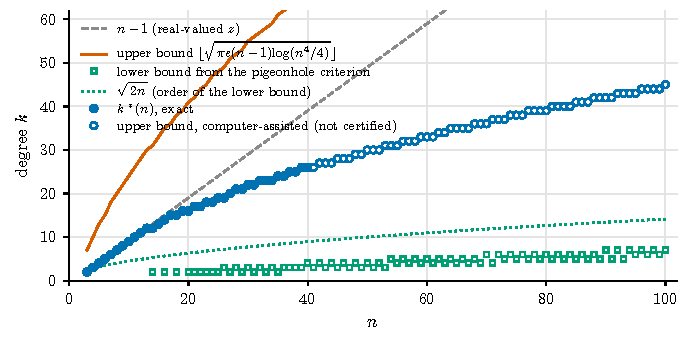
\includegraphics[width=0.72\textwidth]{figures/fig_kstar.pdf}
\caption{The permutation threshold. Exact values of $k^*(n)$ for $3\le n\le40$ (dots), the upper bounds obtained by the exact lattice enumeration for $41\le n\le100$ (open circles), the linear-algebra threshold $n-1$, the bound of \Cref{thm:perm_threshold}(a), and the curve $\sqrt{2n}$, the asymptotic order of the lower bound (b).}
\label{fig:kstar}
\end{figure}

\paragraph{The witnesses.}
The target vectors $\gamma$ were chosen among the shortest vectors of $\Lambda_{n,k^*(n)-1}$ satisfying \eqref{eq:col_feasible}, as produced by the enumeration.
Starting from a semi-magic square of \Cref{lem:twin_squares} (or a Siamese square), a steepest-descent search over exchanges within a row, which fix the row sums, minimised $\sum_j(\text{column sum}_j-M(n)-\gamma_j)^2$, with random exchanges to leave local minima; for the hardest cases a simulated annealing over arbitrary exchanges, with energy the squared distance of both row and column sums to their targets, was used.
We observe (for these $n$ only; this is not a theorem) that for $14\le n\le40$ the threshold is determined by the column-feasibility inequalities alone: $k^*(n)$ is the least $k$ for which no nonzero vector of $\Lambda_{n,k}$ satisfies \eqref{eq:col_feasible}.
Some witnesses come close to the bound of \Cref{lem:col_feasible}: $\max_j|\gamma_j|=924$ against $1014$ at $n=13$, and $24150$ against $24642$ at $n=37$.
Beyond $n=40$ we computed only upper bounds (\Cref{fig:kstar}); for instance $k^*(50)\le30$, $k^*(80)\le39$ and $k^*(100)\le45$.

\subsection{The low-order conditions for \texorpdfstring{$n=3$}{n=3}}

\begin{remark}
\label{rem:n3_lowmode}
Of the $9!$ arrangements of order $3$, exactly $760$ satisfy the degree-$1$ conditions, exactly $72$ (the semi-magic squares) satisfy the degree-$2$ conditions, and exactly $8$ satisfy the degree-$1$ conditions and both diagonal conditions, namely the magic squares (exhaustive enumeration in exact arithmetic).
So $\Elow(S)=0$ if and only if $S$ is magic when $n=3$, although the four conditions are weaker than the magic conditions for real-valued $z$.
The degree-$1$ conditions leave $\gamma=t(1,-2,1)$, $\rho=u(1,-2,1)$; the row, the column and the two diagonals through the centre cover every cell once and the centre four times, which gives $3e=15-2(t+u)$ for the centre value $e$.
We have no proof of $t=u=0$ shorter than the enumeration.
For $n=4$ the equivalence fails (\Cref{rem:four_term_insufficient}); the arrangement there has $\gamma=(3,-9,9,-3)$ and $\rho=(-6,4,10,-8)$, so it satisfies the degree-$2$ condition in $x$ but not in $y$.
\end{remark}

\subsection{Balance of the signed mass}
\label{sec:balance}

Regard $z_c$ as a signed mass at $(x_c,y_c)$.
By \Cref{prop:hierarchy}(a), a semi-magic square balances every separable test function $a(x)+b(y)$, and a magic square also the diagonal indicators; by \Cref{rem:product_inertia} it need not balance $xy$.
For arbitrary arrangements the balance is controlled by the energy:

\begin{remark}[Quantitative balance]
\label{rem:quant_balance}
Since $\sum_cz_cx_c=\sum_jx_j\gamma_j$ and $\sum_jx_j^2=n(n^2-1)/12$, the Cauchy--Schwarz inequality gives
\[
\Bigl|\sum_cz_c(x_c,y_c)\Bigr|^2\le\frac{n(n^2-1)}{12}\bigl(\|\gamma\|^2+\|\rho\|^2\bigr)\le N^2\,\frac{n(n^2-1)}{12}\,\Efull ,
\]
with equality in the first step if and only if $\gamma\parallel(x_j)$ and $\rho\parallel(y_i)$, for instance for $s_{ij}=in+j+1$.
More generally, by \Cref{lem:W_structure}, $\|P_Wz\|^2=n(\|\rho\|^2+\|\gamma\|^2)/N^2+\frac1N\delta^{\mathsf T}\Gamma_D^{-1}\delta$ with $\delta=(\delta_{\mathrm m},\delta_{\mathrm a})$, so $n\Efull\le\|P_Wz\|^2\le\lambda_n\Efull$ with $\lambda_n=n^2/(n-1)$ for odd $n$ and $n^2/(n-2)$ for even $n$; hence $|\sum_cz_c\varphi_c|\le N\|\varphi\|\sqrt{\lambda_n\Efull}$ for every $\varphi\in W$.
\end{remark}

Nonlinear balance is not implied.
With the radial unit vectors $u_c=(x_c,y_c)/|(x_c,y_c)|$ ($u_c=0$ at the centre), each of the eight $3\times3$ magic squares has $|\sum_cz_cu_c|=2(2-\sqrt2)\sqrt5\approx2.62$: for the Lo Shu with rows $(2,7,6),(9,5,1),(4,3,8)$ the edge cells contribute $(-8,4)$ and the corners $(4\sqrt2,-2\sqrt2)$.
For $n=4$ this ring imbalance is positive for all $880$ magic squares (smallest value $0.070$), with mean $5.51$ against $17.06$ for uniformly random arrangements; the magic mean lies at the $7.4$th percentile of the random distribution (\texttt{anc/balance\_check.py}).


\section{The energy of a random arrangement}
\label{sec:random_energy}

Let $S$ be a uniformly random arrangement: $z_c=b_{\pi(c)}$ with $\pi$ uniform and $b$ the centred values $k-\frac{N+1}2$, $1\le k\le N$.
For a test function $\varphi$ put $T_\varphi=\Cov(\varphi,Z)=\sum_ca_cz_c$ with $a_c=(\varphi_c-\bar\varphi)/N$, a linear permutation statistic (\Cref{sec:bg_perm}).
$\Var(\varphi)$ and $\Cov(\varphi,\psi)$ denote population variances and covariances over the $N$ cells, and $\sigma_n^2=(n^2+1)/12$ as in \eqref{eq:sigma}.

\subsection{Means}

\begin{proposition}[Means and covariance structure]
\label{prop:random_energy_moments}
For all test functions $\varphi,\psi$, $\E[T_\varphi]=0$ and $\E[T_\varphi T_\psi]=\sigma_n^2\Cov(\varphi,\psi)$.
Consequently
\begin{gather}
\E\,\Cov(X,Z)^2=\E\,\Cov(Y,Z)^2=\frac{n^4-1}{144},\qquad
\E\,\Cov(\mathbf 1_L,Z)^2=\frac{(n-1)(n^2+1)}{12\,n^2}\ \text{ for every line }L,
\label{eq:single_terms}\\
\E[\Elow]=\frac{(n-1)(n^2+1)(n^3+n^2+12)}{72\,n^2},\qquad
\E[\Efull]=\frac{n^4-1}{6\,n^2}.
\label{eq:mean_low}
\end{gather}
The covariance matrix of the vector of statistics in $\Elow$ (resp.\ $\Efull$) is $\sigma_n^2\Gamma$, with $\Gamma$ the Gram matrix of the centred test functions; its eigenvalues are
\begin{equation}
\Elow:\ \sigma_n^2\Bigl\{\tfrac{n^2-1}{12}\,(\times2),\ \tfrac{n-1}{n^2}\,(\times2)\Bigr\},
\qquad
\Efull:\ \sigma_n^2\Bigl\{\tfrac1n\,(\times\,2n-2),\ \tfrac{n-1}{n^2}\,(\times2),\ 0\,(\times2)\Bigr\}
\label{eq:weights}
\end{equation}
for odd $n$; for even $n$ the pair $\{\tfrac{n-1}{n^2},\tfrac{n-1}{n^2}\}$ is replaced by $\{\tfrac1n,\tfrac{n-2}{n^2}\}$.
\end{proposition}

\begin{proof}
$\sum_ca_c=0$ gives $\E T_\varphi=0$, and \eqref{eq:ww_identity} with $\sum_j b_j^2=N\Var(Z)$ gives $\E[T_\varphi T_\psi]=\frac1{N-1}\cdot\frac{\Cov(\varphi,\psi)}{N}\cdot N\Var(Z)=\sigma_n^2\Cov(\varphi,\psi)$.
The entries of $\Gamma$ follow from \Cref{lem:W_structure}: $\Var(\mathbf 1_L)=(n-1)/n^2$, two lines meeting in $\ell$ cells have covariance $\ell/N-1/n^2$, and $X$, $Y$ are uncorrelated with each other and with the diagonal indicators, since a diagonal meets every row and every column once.
The rows give the block $\frac1n(I-\frac1nJ)$, the columns likewise, and the means are the traces.
\end{proof}

Equivalently, a line sum is the sum of a sample of size $n$ drawn without replacement from $\{1,\dots,N\}$, so $\E\delta_L^2=n\Var(Z)\frac{N-n}{N-1}$.
The means of the two energies coincide if and only if $\frac{n^2-1}{6}=\frac{2(n-1)}{n}$, i.e.\ $n=3$, where both equal $40/27$.

\begin{corollary}[Null distribution of Loly's invariant]
\label{cor:loly_null}
For a uniformly random arrangement, $I(S)$ of \Cref{cor:loly} satisfies
\begin{equation}
\E[I(S)]=\frac{n^{2}(n^{4}-1)}{12},\qquad
\Var\bigl(I(S)\bigr)=N^{2}\sigma_n^{2}\,\Var(X^{2}+Y^{2})=\frac{n^{4}(n^{4}-1)(n^{2}-4)}{1080}.
\label{eq:loly_null}
\end{equation}
The mean equals Loly's value for every distribution of arrangements invariant under relabelling of the values; magic and semi-magic squares sit exactly at the mean, with no fluctuation.
\end{corollary}

\begin{proof}
By \eqref{eq:loly_identity}, $I(S)-\frac{n^2(n^4-1)}{12}=N\,T_{X^2+Y^2}$, so \Cref{prop:random_energy_moments} gives the mean and $\Var(I)=N^2\sigma_n^2\Var(X^2+Y^2)$.
$X$ and $Y$ are independent and uniform on $n$ equally spaced points, so $\Var(X^2+Y^2)=2(\E X^4-(\E X^2)^2)$ with $\E X^2=\frac{n^2-1}{12}$ and $\E X^4=\frac{(n^2-1)(3n^2-7)}{240}$, which gives $\frac{(n^2-1)(n^2-4)}{90}$.
\end{proof}

For $n=3$, $\Var(I)=30$ and $I$ takes $29$ values from $46$ to $74$; for $n=4$, $\Var(I)=2176/3$ and $\Pr(I=340)=13049/450450\approx0.029$ (\texttt{anc/verify\_numbers.py}).

\subsection{Variances}

Write a random energy as a quadratic form $E=\sum_kT_{\varphi_k}^2=z^{\mathsf T}Az$ with $A=\sum_ka_ka_k^{\mathsf T}$, where $a_k=(\varphi_k-\bar\varphi_k)/N$.
$A$ is symmetric with zero row sums.

\begin{theorem}[Variance of a quadratic form in a random arrangement]
\label{thm:var_identity}
Let $A$ be a symmetric $N\times N$ matrix with zero row sums, $N\ge4$, and let $z$ be a uniformly random permutation of the centred values $k-\frac{N+1}2$, $1\le k\le N$.  Then $\E[z^{\mathsf T}Az]=\frac{N(N+1)}{12}\tr A$ and
\begin{equation}
\Var(z^{\mathsf T}Az)=-\frac{N(N+1)(2N+3)}{360}\,(\tr A)^2+\frac{N(N^2-1)(5N+6)}{360}\,\tr(A^2)-\frac{N^2(N+1)^2}{120}\sum_aA_{aa}^2 .
\label{eq:var_identity}
\end{equation}
\end{theorem}

\begin{proof}[Proof (sketch; details in \Cref{sec:app_variance})]
Expand $\E[(z^{\mathsf T}Az)^2]=\sum_{a,b,c,d}A_{ab}A_{cd}\E[z_az_bz_cz_d]$ according to the equality pattern of $(a,b,c,d)$, a set partition of $\{1,2,3,4\}$, and apply M\"obius inversion on the partition lattice, so that each pattern contributes an unrestricted sum.
An unrestricted sum in which some index occurs in only one factor $A_{\cdot\cdot}$ is a row sum of $A$, hence $0$.
Only the four partitions without singletons survive, $12|34$, $13|24$, $14|23$ and $1234$, contributing $(\tr A)^2$, $\tr A^2$, $\tr A^2$ and $\sum_aA_{aa}^2$, with coefficients given by the joint moments of a random permutation of the centred values.
\end{proof}

The identity is a special case of the classical moment formulas for quadratic assignment statistics \cite{mantel1967,hubert1987assignment}.
For the energies the three invariants are explicit; this is where the parity of $n$ enters, through the centre cell shared by the two diagonals when $n$ is odd.

\begin{theorem}[Variances of the energies]
\label{thm:var_closed}
For every $n\ge3$,
\[
\Var(\Elow)=\begin{cases}\dfrac{(n-1)(n^2+1)\,P_{\mathrm o}(n)}{129600\,n^{6}}& n\text{ odd},\\[3mm]
\dfrac{(n^2+1)\,P_{\mathrm e}(n)}{129600\,n^{4}}& n\text{ even},\end{cases}\quad
\Var(\Efull)=\begin{cases}\dfrac{(n-1)(n^2+1)\,Q_{\mathrm o}(n)}{180\,n^{6}}& n\text{ odd},\\[3mm]
\dfrac{(n-2)(n^2+1)\,Q_{\mathrm e}(n)}{180\,n^{5}}& n\text{ even},\end{cases}
\]
where
\begin{align*}
P_{\mathrm o}&=25n^{11}+25n^{10}-82n^9-82n^8-9n^7-1209n^6+3738n^5-5862n^4\\&\qquad+2160n^3-2880n^2-4320n+4320,\\
P_{\mathrm e}&=25n^{10}-107n^8+73n^6-1200n^5+4947n^4-9600n^3+13782n^2-13680n+10080,\\
Q_{\mathrm o}&=5n^6-5n^5-17n^4+11n^3-24n^2+18n+6,\qquad
Q_{\mathrm e}=5n^5-12n^3+12n^2-23n+12 .
\end{align*}
For both parities,
\[
\Var(\Elow)=\frac{n^8}{5184}-\frac{41\,n^6}{64800}+O(n^4),\qquad
\Var(\Efull)=\frac{n^3}{36}-\frac{n^2}{18}-\frac{7n}{180}+O(1).
\]
\end{theorem}

\begin{proof}
\Cref{thm:var_identity} with $N=n^2$ and the invariants \eqref{eq:inv_low}--\eqref{eq:inv_full} of \Cref{sec:app_variance}; the expansions follow.
\end{proof}


At $n=3$ the formulas give $\Var(\Elow)=1532/2187$ and $\Var(\Efull)=398/2187$, the values obtained by enumerating all $9!$ arrangements.

\subsection{Limit law}

\begin{corollary}[Limit law]
\label{cor:random_energy_clt}
Let $\tau_1^2,\dots,\tau_4^2$ be the variances of $T_X,T_Y,T_{D_{\mathrm m}},T_{D_{\mathrm a}}$ (the diagonal of $\sigma_n^2\Gamma$).
As $n\to\infty$, $\bigl(T_X/\tau_1,T_Y/\tau_2,T_{D_{\mathrm m}}/\tau_3,T_{D_{\mathrm a}}/\tau_4\bigr)$ converges in distribution to a standard Gaussian vector in $\R^4$, and
\begin{equation}
\frac{\Elow}{\E[\Elow]}\ \xrightarrow{\ d\ }\ \mathrm{Exp}(1).
\label{eq:low_limit}
\end{equation}
\end{corollary}

\begin{proof}
Fix $\alpha\in\R^4\setminus\{0\}$ and let $a=\sum_k\alpha_ka_k/\tau_k$ be the corresponding combination of the four centred, standardised test vectors.
Then $\sum_k\alpha_kT_k/\tau_k=\sum_ca_cz_c$ is a linear permutation statistic with doubly centred array $d(c,v)=a_cb_v$, and
\[
\frac{\max_{c,v}|a_cb_v|}{\bigl(N^{-1}\sum_{c,v}a_c^2b_v^2\bigr)^{1/2}}=\frac{\max_c|a_c|}{\|a\|_2}\cdot\frac{\max_v|b_v|}{(\sum_vb_v^2/N)^{1/2}} .
\]
The second factor tends to $\sqrt3$.
For the first, $\max_c|a_c|\le\sum_k|\alpha_k|\max_c|a_{k,c}|/\tau_k$, and $\max_c|a_{k,c}|/\|a_k\|_2$ is $O(n^{-1})$ for $X$ and $Y$ and $O(n^{-1/2})$ for a diagonal indicator (a centred indicator of $n$ of the $N$ cells); moreover $\|a\|_2^2$ is proportional to $\alpha^{\mathsf T}C_n\alpha$ with $C_n$ the correlation matrix, which tends to the identity because the only nonzero correlation is $\operatorname{corr}(T_{D_{\mathrm m}},T_{D_{\mathrm a}})=-1/(n-1)$ for even $n$.
So the quotient tends to $0$, Hoeffding's theorem (\Cref{sec:bg_perm}) gives asymptotic normality of every such combination, and the Cram\'er--Wold device gives the joint limit $N(0,I_4)$.
In $\Elow=\tau_1^2(\tilde T_X^2+\tilde T_Y^2)+\tau_3^2\tilde T_{D_{\mathrm m}}^2+\tau_4^2\tilde T_{D_{\mathrm a}}^2$ (tildes denoting standardised statistics) the diagonal weights satisfy $\tau_3^2/\tau_1^2=12(n-1)/(n^2(n^2-1))\to0$, so $\Elow/(2\tau_1^2)\to\frac12\chi^2_2=\mathrm{Exp}(1)$; and $\E[\Elow]/(2\tau_1^2)\to1$.
\end{proof}

\begin{remark}[Gaussian approximation at finite $n$]
\label{rem:gauss_mixture}
The Gaussian approximation replaces an energy by $\sum_jw_j\chi^2_{1,j}$, with independent $\chi^2_1$ variables and weights $w_j$ the eigenvalues \eqref{eq:weights}; its density can be computed by inversion of the characteristic function \cite{imhof1961} (\Cref{fig:random_energy}).
It has the exact mean but variance $2\sum_jw_j^2$, and by \Cref{thm:var_closed} the ratio of the exact variance to this value is
\[
1-\frac2n-\frac{7}{5n^2}+O(n^{-3})\quad(\Efull),\qquad 1-\frac{82}{25n^2}+O(n^{-3})\quad(\Elow);
\]
the deficit comes from the two negative terms of \eqref{eq:var_identity}.
For $\Efull$ the number of statistics grows with $n$ and \Cref{cor:random_energy_clt} does not apply.
The approximation is poor for small $n$: at $n=3$ the Gaussian standard deviation of $\Efull$ is about twice the exact one (\Cref{tab:random_energy}).
\end{remark}

\begin{table}[htbp]
\centering
\small
\begin{tabular}{c l r r r r}
\toprule
$n$ & energy & $\E[E]$ & $\sqrt{\Var E}$ & Gaussian sd & variance ratio \\
\midrule
3 & $\Elow$  & $40/27$ & 0.8370 & 1.171 & 0.511 \\
3 & $\Efull$ & $40/27$ & 0.4266 & 0.869 & 0.241 \\
4 & $\Elow$  & $391/96$ & 3.1284 & 3.586 & 0.761 \\
4 & $\Efull$ & $85/32$ & 0.9074 & 1.349 & 0.453 \\
5 & $\Elow$  & $234/25$ & 8.0483 & 8.694 & 0.857 \\
5 & $\Efull$ & $104/25$ & 1.3966 & 1.867 & 0.560 \\
6 & $\Elow$  & $2035/108$ & 17.122 & 18.007 & 0.904 \\
6 & $\Efull$ & $1295/216$ & 1.9671 & 2.459 & 0.640 \\
7 & $\Elow$  & $5050/147$ & 32.174 & 33.349 & 0.931 \\
7 & $\Efull$ & $400/49$ & 2.5697 & 3.089 & 0.692 \\
8 & $\Elow$  & $22295/384$ & 55.377 & 56.888 & 0.948 \\
8 & $\Efull$ & $1365/128$ & 3.2352 & 3.777 & 0.734 \\
\bottomrule
\end{tabular}
\caption{Exact means and standard deviations of the two energies (\Cref{prop:random_energy_moments}, \Cref{thm:var_closed}), the standard deviation of the Gaussian approximation of \Cref{rem:gauss_mixture}, and the ratio of the exact to the Gaussian variance.}
\label{tab:random_energy}
\end{table}

\begin{figure}[htbp]
\centering
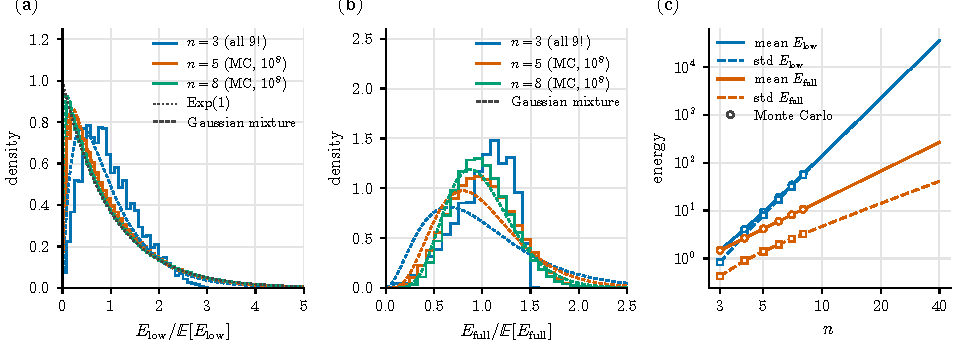
\includegraphics[width=0.92\textwidth]{figures/fig_random_energy.pdf}
\caption{Energy of a uniformly random arrangement. (a)~Distribution of $\Elow/\E[\Elow]$ for $n=3$ (all $9!$ arrangements) and $n=5,8$ ($10^8$ Monte Carlo samples each), with the densities of the Gaussian approximation (dashed) and the limit $\mathrm{Exp}(1)$ of \Cref{cor:random_energy_clt} (dotted). (b)~The same for $\Efull$, where the Gaussian approximation improves slowly (\Cref{rem:gauss_mixture}). (c)~Exact mean (solid) and standard deviation (dashed) of both energies for $3\le n\le40$, with Monte Carlo values for $3\le n\le8$ (open markers).}
\label{fig:random_energy}
\end{figure}


\section{Computations for small orders}
\label{sec:computations}

All counts below were computed in exact integer arithmetic; the methods are described in \Cref{sec:appendix}, and every number is produced by a script in the ancillary directory \texttt{anc/}.

\subsection{The low-order class for \texorpdfstring{$n=4$}{n=4}}
\label{sec:lowmode_n4}

Let $L_n$ be the set of arrangements with $\Elow=0$, i.e.\ $\Cov(X,Z)=\Cov(Y,Z)=0$ and both diagonal sums equal to $M(n)$.
With cells indexed by $(i,j)$, these are the conditions $U_1=U_2=\frac{n-1}2\cdot\frac{N(N+1)}2$ and $U_3=U_4=M(n)$ on the sums
$U_1=\sum_{i,j}j\,s_{ij}$, $U_2=\sum_{i,j}i\,s_{ij}$, $U_3=\sum_is_{ii}$, $U_4=\sum_is_{i,n-1-i}$, which are additive over cells.

\begin{proposition}[The size of $L_4$]
\label{prop:L4}
$|L_3|=8$ (the magic squares), and
\[
|L_4|=14{,}639{,}440=8\times1{,}829{,}930,
\]
of which $7{,}040$ are magic squares.
The class $\{\Cov(X,Z)=\Cov(Y,Z)=0\}$ has $6{,}697{,}177{,}424$ members for $n=4$, and the class with both diagonal sums equal to $34$ has $49{,}932{,}288{,}000$.
\end{proposition}

\begin{proof}[Computation]
A meet-in-the-middle enumeration over $(U_1,\dots,U_4)$, splitting the grid into the top two and bottom two rows (\Cref{sec:appendix}); the matching pairs were expanded to obtain the breakdown of \Cref{tab:L4}.
The same program reproduces the brute-force counts for $n=3$ ($8$, $760$, $4224$, and $72$ semi-magic squares) and, with the $2n$ line sums in place of $U_1,U_2$, the $7{,}040$ magic and $549{,}504$ semi-magic squares of order $4$.
The diagonal-only count also follows from a direct count: there are $2150$ ordered pairs of disjoint $4$-subsets of $\{1,\dots,16\}$ with sum $34$, and $2150\cdot(4!)^2\cdot8!=49{,}932{,}288{,}000$.
\end{proof}

Since $D_4$ acts freely on the set of all arrangements (entries are distinct) and preserves $L_4$, $L_4$ consists of $1{,}829{,}930$ orbits of size $8$.

\begin{table}[htbp]
\centering
\small
\begin{tabular}{lrrrr}
\toprule
 & \multicolumn{4}{c}{columns with sum 34} \\
\cmidrule(lr){2-5}
rows with sum 34 & 0 & 1 & 4 & total \\
\midrule
0 & 9\,637\,312 & 2\,172\,824 & 100\,728 & 11\,910\,864 \\
1 & 2\,172\,824 & 429\,312 & 9\,336 & 2\,611\,472 \\
4 & 100\,728 & 9\,336 & \textbf{7\,040} (magic) & 117\,104 \\
\midrule
total & 11\,910\,864 & 2\,611\,472 & 117\,104 & 14\,639\,440 \\
\bottomrule
\end{tabular}
\caption{The members of $L_4$ by the number of rows and of columns with sum $M(4)=34$; the table is symmetric under transposition.}
\label{tab:L4}
\end{table}

Exactly two or three rows with sum $34$ are impossible in $L_4$: the row deviations $e_i$ satisfy $\sum_ie_i=0$ and $\sum_iie_i=0$, which cannot hold with exactly one or two nonzero $e_i$; the same holds for columns.
Thus $7040/14{,}639{,}440\approx0.048\%$ of $L_4$ is magic, and $9{,}637{,}312$ members ($66\%$) have no row or column with sum $34$, among them the arrangement of \Cref{rem:four_term_insufficient}.

\paragraph{A local-limit estimate.}
Under a uniformly random arrangement the vector $(U_1,\dots,U_4)$ has mean equal to the target vector and covariance matrix $\Sigma_U$ given by \eqref{eq:ww_identity}: $U_1,U_2$ are uncorrelated with each other and with the diagonal sums, which have correlation $-1/(n-1)$ for even $n$ and $0$ for odd $n$.
The single transpositions change $(U_1,\dots,U_4)$ by vectors whose $\Z$-span is $\Z^4$ (Smith normal form, $n\le8$).
A Gaussian local limit would therefore give $|L_n|\approx N!\,(2\pi)^{-2}\det(\Sigma_U)^{-1/2}$.
This estimate is $13.6$ for $n=3$ ($|L_3|=8$) and $1.82\times10^{7}$ for $n=4$, so $|L_4|$ is $0.80$ times the estimate; for the two-condition classes the ratios at $n=3,4$ are $0.59,0.91$ (first moments) and $1.10,0.96$ (diagonals).
For $n=5,6$ Monte Carlo ($10^{10}$ and $2\times10^{10}$ samples, $328$ and $62$ members of $L_n$) gives $|L_5|\approx5.1\times10^{17}$ ($\pm6\%$) and $|L_6|\approx1.2\times10^{33}$ ($\pm13\%$), ratios $0.76$ and $0.78$ to the estimate.
Since $\det(\Sigma_U)^{1/2}$ grows like $n^{13}$, one expects $|L_n|/N!$ to decay like $n^{-13}$, and the fraction of magic squares in $L_n$ to tend to $0$; local limit theorems for permutation statistics of this kind are studied in \cite{kuperberg2017probabilistic,eberhard2019additive}, and related counts of matrices with prescribed margins in \cite{canfield2010asymptotic}.

\subsection{Single swaps}
\label{sec:swap-gaps}

\begin{remark}[Single-swap formula]
\label{rem:swap}
Let $S^{ab}$ be obtained from $S$ by exchanging the entries of cells $a\ne b$, let $d=s_b-s_a$, let $\lambda(a,b)$ be the number of lines containing exactly one of $a,b$, and $u_S(c)=\sum_{L\ni c}\delta_L(S)$.
Expanding \eqref{eq:Efull_devs},
\[
N^{2}\bigl(\Efull(S^{ab})-\Efull(S)\bigr)=d^{2}\lambda(a,b)+2d\bigl(u_S(a)-u_S(b)\bigr),
\]
the incremental evaluation used in local search \cite{pinn1998number}.
Here $\lambda(a,b)=2[i\ne i']+2[j\ne j']+[\text{a diagonal separates }a,b]+[\text{the other diagonal separates }a,b]\in\{2,\dots,6\}$ for $a=(i,j)$, $b=(i',j')$.
For a magic square $S$, $N^2\Efull(S^{ab})=d^2\lambda(a,b)\ge2$, so no two magic squares differ by a transposition, and the values lie in the set $\{d^2\lambda:1\le d\le N-1,\ 2\le\lambda\le6\}$.
The smallest value $g_{\min}(S)=\min_{a\ne b}d^2\lambda(a,b)$ satisfies $2\le g_{\min}(S)\le6$: the value $2$ occurs if and only if two consecutive values lie in a common row or column and off both diagonals, and consecutive values give at most $6$.
\end{remark}

Over the $880\cdot\binom{16}2=105{,}600$ swaps of the $880$ magic squares of order $4$ up to $D_4$, the gap $d^2\lambda$ takes $70$ values from $2$ to $980$, and $g_{\min}(S)$ is $2$ for $432$ squares, $3$ for $420$ and $4$ for $28$ (\Cref{fig:swap_spectrum}); it is $3$ for the magic squares of order $3$.
For $n=3$, besides the eight magic squares, $\Efull$ has eight non-magic local minima with respect to swaps, all with $N^2\Efull=2$; $\Elow$ has $344$ local minima, of which $336$ are non-magic.
Steepest swap descent on $\Efull$ from a random arrangement reaches a magic square in $19.5\%$ of runs for $n=4$, $1.2\%$ for $n=5$ and $0.8\%$ for $n=6$ (\texttt{anc/algorithms.py}).

\begin{figure}[htbp]
\centering
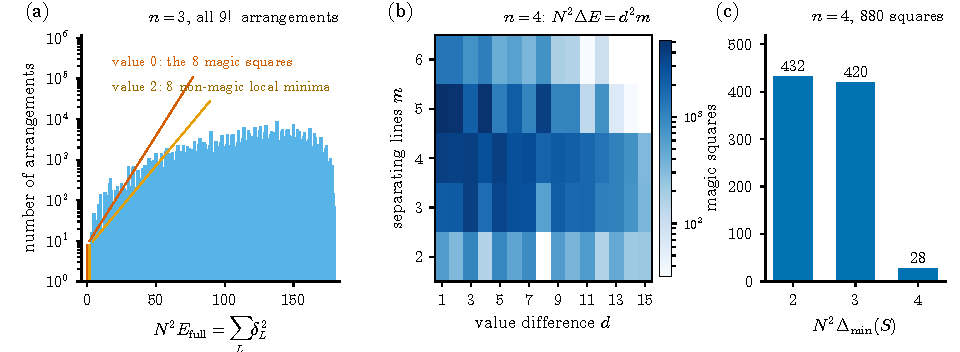
\includegraphics[width=\textwidth]{figures/fig_swap_spectrum.pdf}
\caption{Swap gaps. (a)~For $n=3$, the number of arrangements with each value of $N^2\Efull=\sum_L\delta_L^2$; the eight magic squares are at $0$ and the eight non-magic local minima at $2$. (b)~For $n=4$, the number of single swaps of the $880$ magic squares ($105{,}600$ in total) by value difference $d$ and number $\lambda$ of separating lines; the gap is $d^2\lambda$. (c)~The smallest gap $g_{\min}(S)$ over the $880$ squares.}
\label{fig:swap_spectrum}
\end{figure}


\section{Open questions}
\label{sec:discussion}

The main results are the two-sided bound $(\sqrt2-o(1))\sqrt n\le k^*(n)\le(2\sqrt{\pi e}+o(1))\sqrt{n\log n}$ for the permutation threshold, with exact values for $n\le40$ (computer-assisted for the upper bounds when $18\le n\le40$), and exact second moments of the line-sum energies of a random arrangement.
The following questions remain.

\begin{enumerate}\setlength\itemsep{2pt}
\item \emph{The order of $k^*(n)$.} Is $k^*(n)\asymp\sqrt n$?
The upper bound uses only that $\gamma$ is a nonzero integer vector with $\|\gamma\|_1\le n^4/4$.
In that class the pigeonhole principle produces, for all large $n$, vectors vanishing to order $\ge\lfloor2\sqrt n\rfloor$ at $1$ (\Cref{sec:kstar_upper}), so a bound of smaller order than $\sqrt n$ needs more information about $\gamma$.
Whether the order $\sqrt{n\log n}$ of \Cref{lem:jensen} is attained within this class is, as far as we know, open; this is separate from realisability, i.e.\ which such vectors are column deviations of arrangements.
For $14\le n\le40$, $k^*(n)$ is the least $k$ for which $\Lambda_{n,k}$ contains no nonzero vector satisfying \eqref{eq:col_feasible} (\Cref{sec:kstar_exact}).  Is this true for all $n$, and is $k^*(n)$ nondecreasing?
\item \emph{The size of $L_n$.} Is $|L_n|\sim N!\,(2\pi)^{-2}\det(\Sigma_U)^{-1/2}\,c_n$ with $c_n$ bounded away from $0$ and $\infty$, i.e.\ does a local limit theorem hold for the four statistics $(U_1,\dots,U_4)$ of \Cref{sec:lowmode_n4}?  The ratio $c_n$ is $0.59$, $0.80$ for $n=3,4$ and about $0.76$, $0.78$ for $n=5,6$.
\item \emph{Other families.} The orthogonality formulation applies to pandiagonal and Franklin squares \cite{loly2007franklin}, with $W$ replaced by the span of the relevant line indicators.  The corresponding thresholds and random energies have not been worked out.
\end{enumerate}


\section*{Acknowledgments}
\label{sec:ai_statement}

Large language models (Anthropic's Claude and Google's Gemini) were used to assist with mathematical exploration, software implementation, and manuscript editing; all proofs and exact computational certificates have been verified by the author, who takes full responsibility for the content.


\bibliographystyle{plain}
\bibliography{references}

\appendix
\section{Computational methods}
\label{sec:appendix}

\paragraph{Hardware and software.}
All computations were run on an Apple M4 Max (16 cores, 128\,GB) under macOS, with Python 3.9.6, NumPy 2.0.2, SciPy 1.13.1 and C code compiled with Apple clang 17.
Uniformly random arrangements were generated by Fisher--Yates shuffles (NumPy's default generator; \texttt{xoshiro256**} in C); the Monte Carlo of \Cref{tab:random_energy} uses $10^8$ arrangements per order.
All energies are evaluated from \eqref{eq:Efull}.
The exact statements of \Cref{sec:theory} and the numbers quoted in \Cref{sec:results} are checked in exact integer or rational arithmetic by \texttt{anc/verify\_numbers.py}: the $n=3$ enumeration, all $105{,}888$ single swaps of the $880+8$ magic squares of orders $4$ and $3$ and the swaps of the Siamese squares, the exact means and variances for $n=3,\dots,6$, the null distribution of Loly's invariant, the witnesses, the product-of-inertia values, and the data for \Cref{sec:lowmode_n4}.
The numerical statements of \Cref{sec:balance} are produced by \texttt{anc/balance\_check.py}.

\paragraph{Exact moments and variances.}
The means in \Cref{prop:random_energy_moments} are traces of the covariance matrix $\sigma_n^2G$.
The variances were computed as exact rationals for each $n\le45$ by expanding $\E[E^2]$ over the $15$ equality patterns of a cell quadruple, with the fourth-moment expectations of the uniform permutation expressed through the power sums $p_2,p_4$ of the centred values; the rational functions \eqref{eq:var_low} were then obtained by interpolation separately for odd and even $n$ and verified on $5$--$11$ further orders each, and against the exhaustive $n=3$ values.
Densities of the Gaussian-limit mixtures in \Cref{fig:random_energy} were computed by numerical inversion of the characteristic function, the method of Imhof \cite{imhof1961}.

\paragraph{Meet-in-the-middle enumeration of $L_4$.}
The four statistics $T_1=\sum_{ij}j\,s_{ij}$, $T_2=\sum_{ij}i\,s_{ij}$, $T_3=\sum_i s_{ii}$, $T_4=\sum_i s_{i,n-1-i}$ are additive over cells.
The $16$ cells are split into the top two rows $A$ and the bottom two rows $B$.
For each of the $\binom{16}{8}=12{,}870$ value sets $V$ and each of the $8!$ bijections $V\to A$ the partial vector $(T_1,\dots,T_4)|_A$ is packed into a $27$-bit key; for the complementary set and each bijection $V^c\to B$ the key of (target $-$ partial) is formed; the two key lists are sorted and merged, and the sum over matching keys of the product of multiplicities is $|L_4|$.
This touches $2\times12{,}870\times40{,}320\approx1.04\times10^9$ partial vectors instead of $16!\approx2.1\times10^{13}$ arrangements and runs in $9$\,s on $16$ threads.
Matching pairs are expanded explicitly to obtain the $14{,}639{,}440$ members, which are then classified by row and column sums and by $D_4$-orbit.
Validation is described after \Cref{prop:L4}.

\paragraph{Reproducibility.}
The scripts for every table and figure, the C enumerator and Monte Carlo code, the verification scripts and the JSON files containing the reported numbers are provided as ancillary files in \texttt{anc/}, with a \texttt{README} listing the commands that regenerate them.


\section{Variance closed forms}
\label{sec:app_variance}

For a uniformly random arrangement the variances of the two energies of \Cref{prop:random_energy_moments} are rational
functions of $n$ of the form
\begin{equation}
\begin{aligned}
\Var(\Elow)&=\frac{(n-1)(n^2+1)\,P_{\mathrm o}(n)}{129600\,n^{6}}\ (n\ \text{odd}),&\quad
&\frac{(n^2+1)\,P_{\mathrm e}(n)}{129600\,n^{4}}\ (n\ \text{even});\\
\Var(\Efull)&=\frac{(n-1)(n^2+1)\,Q_{\mathrm o}(n)}{180\,n^{6}}\ (n\ \text{odd}),&\quad
&\frac{(n-2)(n^2+1)\,Q_{\mathrm e}(n)}{180\,n^{5}}\ (n\ \text{even}),
\end{aligned}
\label{eq:var_low}
\end{equation}
with integer polynomials $P_{\mathrm o}$, $P_{\mathrm e}$ of degrees $11$, $10$ and leading coefficient $25$, and
$Q_{\mathrm o}$, $Q_{\mathrm e}$ of degrees $6$, $5$ and leading coefficient $5$, so that $\Var(\Elow)=n^8/5184+O(n^7)$ and
$\Var(\Efull)=n^3/36+O(n^2)$.  The polynomials are listed in the ancillary file \texttt{anc/data\_witnesses\_variances.json}
(and in \texttt{anc/variance\_fits.json}); they were obtained as described in \Cref{sec:appendix}, and at $n=3$ they
give $1532/2187$ and $398/2187$, the exhaustive values, at $n=4$ $14093/1440$ and $527/640$ (\Cref{tab:random_energy}).

\section{A witness for \texorpdfstring{$k^*(5)=4$}{k*(5)=4}}
\label{sec:app_witnesses}

The arrangement
\[
\begin{pmatrix}1&22&11&24&7\\23&3&12&2&25\\18&6&19&17&5\\4&21&14&10&16\\20&9&15&8&13\end{pmatrix}
\]
has all row sums equal to $M(5)=65$ and column sums $66,61,71,61,66$, i.e.\ $\gamma=(1,-4,6,-4,1)=\bigl((-1)^j\binom4j\bigr)_j$;
by \eqref{eq:finite_diff} it satisfies the degree-$3$ conditions of \Cref{def:degree_k} without being semi-magic, so
$k^*(5)=4$.  The analogous witnesses for $6\le n\le13$ (\Cref{rem:kstar_search}) are in the ancillary file
\texttt{anc/data\_witnesses\_variances.json}; \texttt{anc/verify\_numbers.py} verifies them.



\end{document}
